%%%% CAPÍTULO 3 - MATERIAL E MÉTODOS (PODE SER OUTRO TÍTULO DE ACORDO COM O TRABALHO REALIZADO)
%%
%% Deve apresentar o modelo utilizado, a modelagem
%% empregada, as simplificações necessárias, a
%% metodologia e a descrição do método de cálculo 
%% utilizado no desenvolvimento da pesquisa para que
%% a mesma possa ser reconstituída. Deve ainda 
%% apresentar resultados de amostras e comentários.
%% Deve apresentar a descrição da montagem 
%% experimental, metodologia para a obtenção de 
%% resultados, análise de erros, amostra de resultados
%% obtidos e comentários. Atenção: Esta parte pode ser
%% subdividida em mais capítulos de acordo com a 
%% especificidade do assunto.

%% Título e rótulo de capítulo (rótulos não devem conter caracteres especiais, acentuados ou cedilha)
\chapter{Metodologia}
\label{cap:materialemetodos}

\section{Transporte coletivo de ônibus}

\ric{Dar ênfase no problema. Quais são os elementos principais do transporte de ônibus a ser modelado neste trabalho. Depois pode exemplicar com o transporte de Curitiba.}

\definecolor{clauciane}{RGB}{204, 0 ,0}

\definecolor{courb2020}{RGB}{0, 204 ,0}

Segundo o Instituto de Pesquisa e Planejamento Urbano de Curitiba (IPPUC), o sistema de transporte coletivo de Curitiba é composto por linhas urbanas e metropolitanas. Estas linhas são caracterizadas quanto a sua função e categoria, sendo diferenciadas por cores, conforme ilustra a Figura ~\ref{fig:linhas}. 

Segue uma breve descrição de cada linha ofertada~\cite{Cur:19}:

\begin{itemize}
    \item Expresso Ligeirão: Linhas operadas por veículos biarticulados nas cores azul e vermelha com capacidade para 250 passageiros. Caracterizada por deslocamentos mais rápidos em canaletas exclusivas e número reduzido de paradas, os embarques e desembarques do Expresso Ligeirão são realizados em terminais e estações-tubo. 

    \item Expresso: São linhas operadas por veículos tipo biarticulados, na cor vermelha, com capacidade para até 170 passageiros. As linhas Expresso ligam os terminais de integração ao centro da cidade, através das canaletas exclusivas. Embarques e desembarques são feitos em nível nos terminais e nas estações-tubo existentes no trajeto.

    \item Linha Direta (Ligeirinho): Linhas operadas com veículos nas cores prata ou cinza.  Os veículos operantes nas linhas diretas realizam com paradas em média a cada 3 km, com embarque e desembarque em nível nas estações-tubo. As linhas diretas são linhas complementares, principalmente das linhas expressas e interbairros.

    \item Interbairros: São linhas que ligam os diversos bairros e terminais sem passar pelo Centro da cidade. Operadas por veículos tipo padron ou articulados, na cor verde.
    
    \item Alimentador: São operadas por veículos tipo micro, comum ou articulados, nas cores laranja ou amarela. As linhas alimentadoras são responsáveis pela conexão dos terminais de integração aos bairros de cada região.

    \item Troncal: As linhas troncais ligam os terminais de integração ao Centro da cidade, utilizando vias compartilhadas. Operam com veículos tipo padron ou articulados, nas cores amarela ou laranja. 

    \item Convencional: Sem a realização de integração, as linhas convencionais ligam os bairros ao Centro da cidade. Operam com veículos tipo micro ou comum, nas cores amarela ou laranja.
        
    \item Circular Centro:  A linha circular centro atende os principais pontos atrativos da região central de Curitiba, tais como praças, shoppings, Rodoviária e Biblioteca Pública. É operada com veículos tipo micro-ônibus e apresenta tarifa diferenciada.

    \item Linha Turismo: Linha caracterizada pela realização do trajeto de turismo urbano de Curitiba. Passa pelos principais parques e pontos turísticos da cidade (tarifa diferenciada). Com saída do Centro, os ônibus da linha turismo são to tipo double deck e são da cor verde claro.

\end{itemize}

 \begin{figure}[!h]
 \caption{Composição da frota}
     \centering
     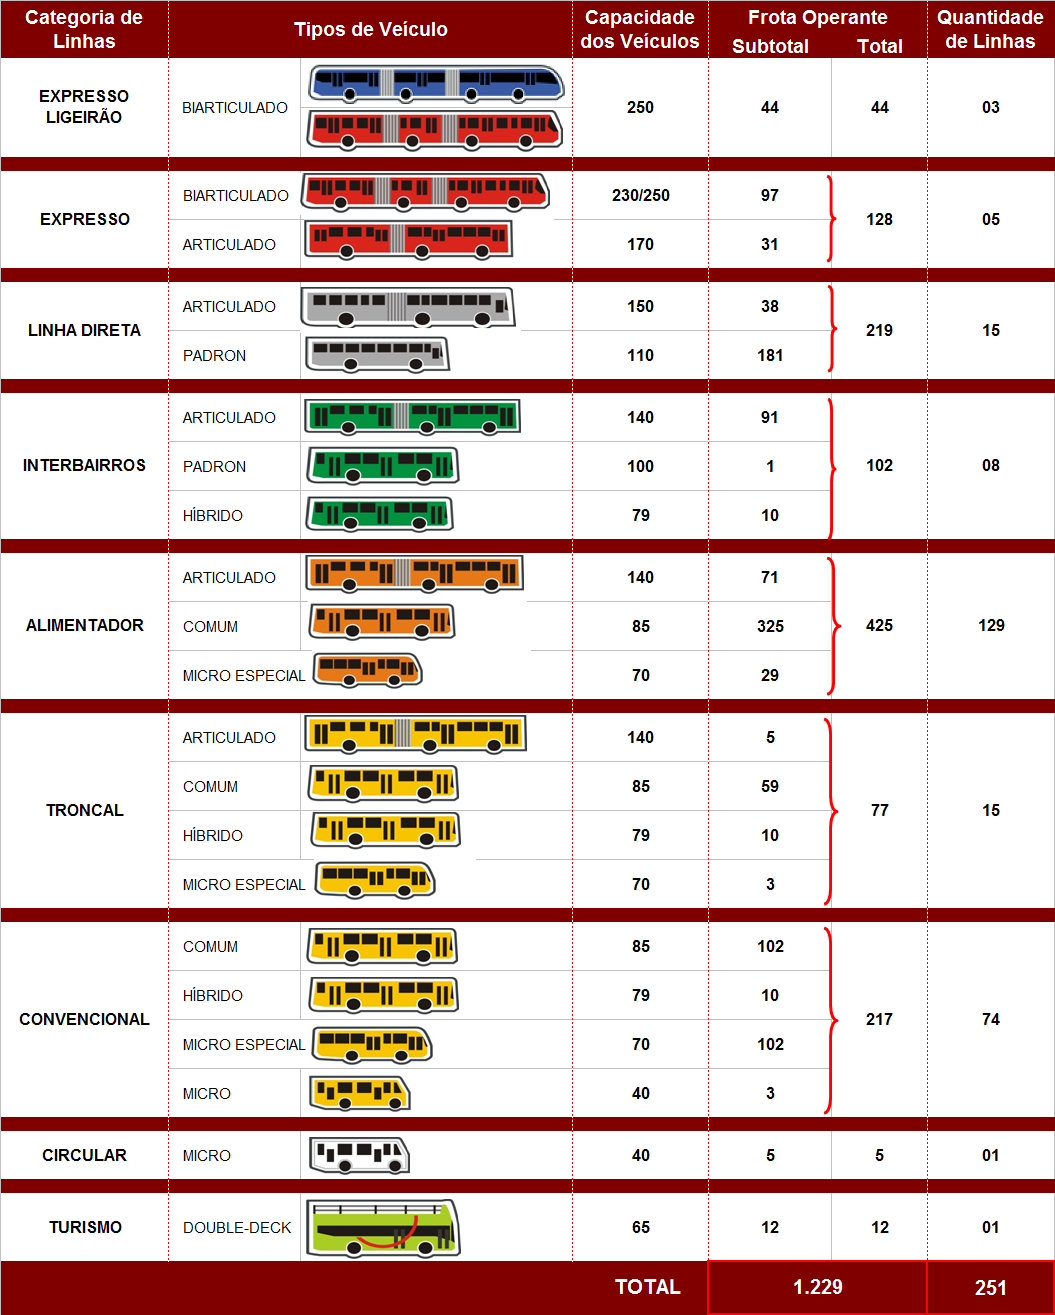
\includegraphics[scale=.40]{./Capitulo3/img/composicao-frota.png}
         \label{fig:linhas}
     \fonte{Rede Integrada de Transporte~\cite{Cur:19}}
 \end{figure}


Os terminais, assim como as linhas do transporte público são divididas em categorias e  recebem uma classificação sendo divididos em: terminais de ponta, terminais intermediários, terminais de bairros, terminais de área central e terminais metropolitanos. Tal divisão, como o nome sugere, indica a posição dos mesmos no sistema de transporte, conforme ilustra a Figura ~\ref{fig:terminais}.
 \begin{figure}[!h]
 \caption{Localização e classificação dos terminais de ônibus de Curitiba}
     \centering
     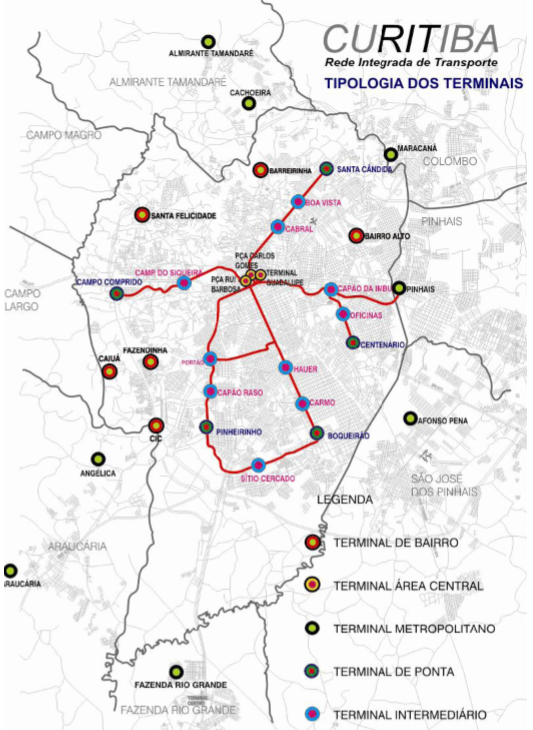
\includegraphics[scale=.95]{./Capitulo3/img/terminais.png}
         \label{fig:terminais}
     \fonte{Plano de Mobilidade Urbana de Curitiba, IPUCC 2019}
 \end{figure}

\section{Um modelo do transporte de ônibus via grafo temporal} \label{sec:met}
%\section{Modelo Proposto} \label{sec:met}


O modelo proposto para o transporte público de Curitiba é mostrado na Figura~\ref{fig:model}. Este modelo tem por base o modelo de~\cite{wach:19}.

A Figura~\ref{fig:model} apresenta um grafo com vértices temporais (\emph{Line} e \emph{Trip} ) e espaço-temporais (\emph{BusStop} e \emph{Event}). Os vértices temporais carregam informações que variam com o tempo, enquanto os vértices espaço-temporais possuem informações de tempo associadas a dados de posicionamento georreferenciado. Vértices adicionais definem propriedades estáticas inerentes à operação de transporte público de Curitiba(\emph{Timetable}, \emph{ServiceCategory}, \emph{Color}, \emph{BusStopType} e \emph{Neighbourhood}), assim como agrupamentos temporais do modelo que permitem recuperar informações para diferentes escalas de tempo (\emph{Year}, \emph{Month}, \emph{Day} e \emph{Hour}). Em resumo, o modelo da Figura~\ref{fig:model} representa dependências temporais e espaço-temporais entre os vértices do grafo que descreve a operação de um sistema de transporte.

 \begin{figure}[!h]
 \caption{Modelo TVG da movimentação dos ônibus do transporte.}
     \centering
     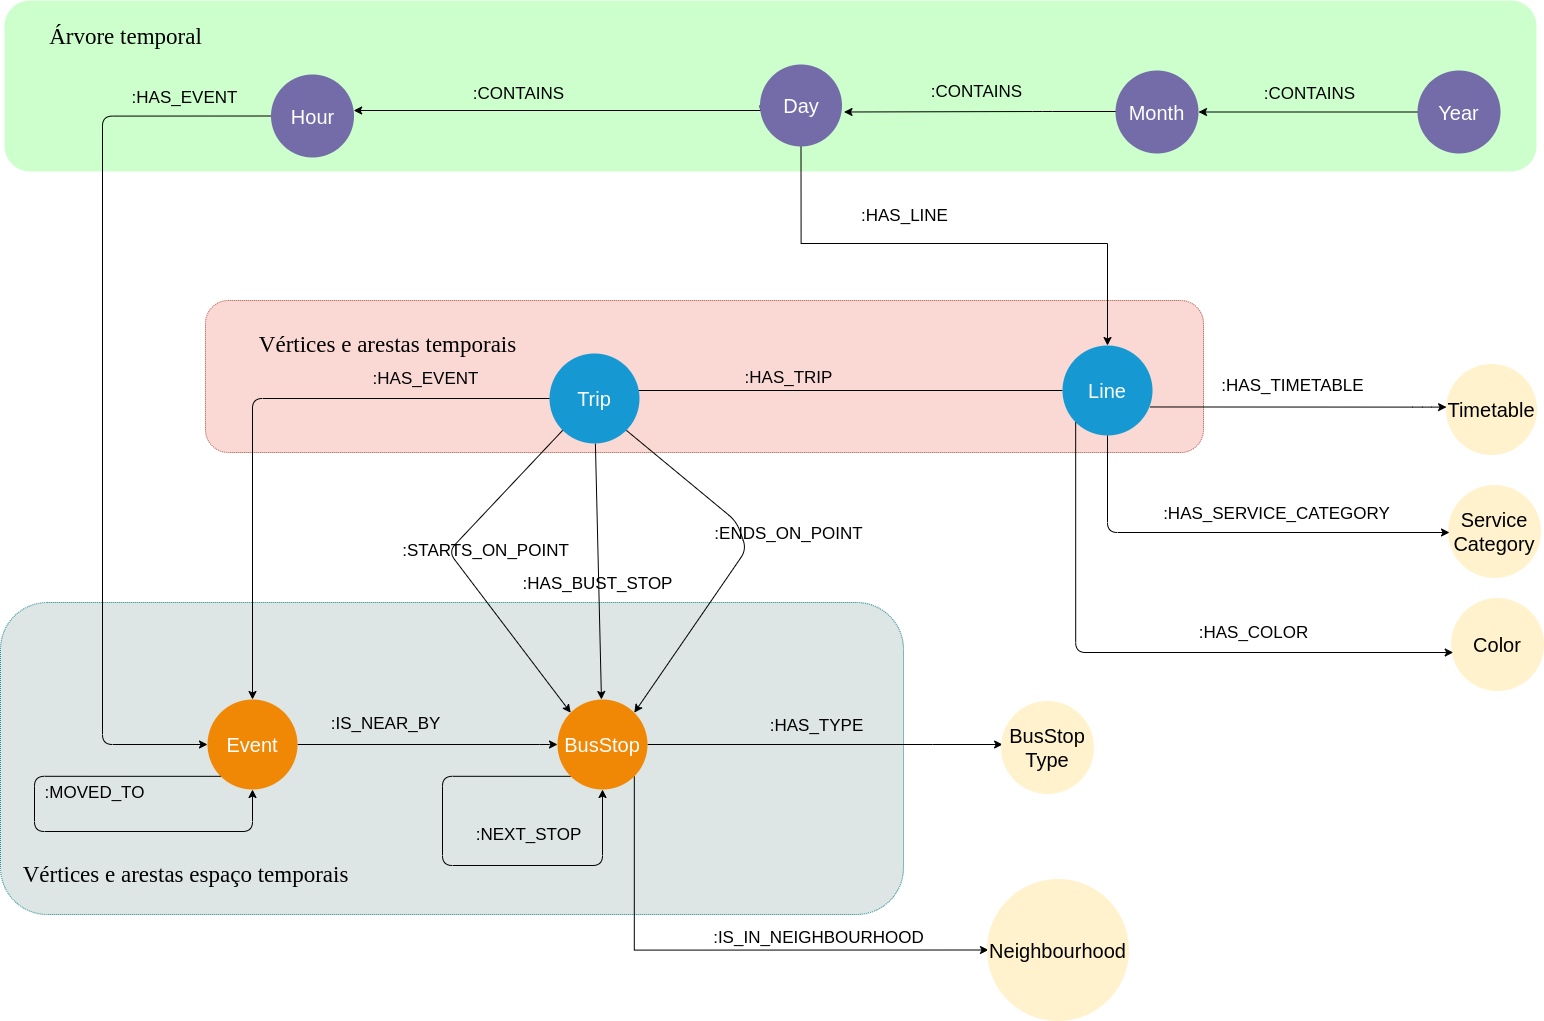
\includegraphics[scale=.25]{./Capitulo3/img/graph-model.png}
         \label{fig:model}
     \fonte{Autoria própria}
 \end{figure}
 
 

Os atributos dos vértices do grafo da Figura~\ref{fig:model} são mostrados nas Tabelas~\ref{tab:vertice_line}, \ref{tab:vertice_trip}, \ref{tab:vertice_busstop}, \ref{tab:vertice_event}, \ref{tab:vertice_color}, \ref{tab:vertice_service_category}, \ref{tab:vertice_busstop_type},\ref{tab:vertice_timetable} e \ref{tab:vertice_neighbourhood}. 

Cada linha de ônibus (vértices \emph{Line} - Tabela~\ref{tab:vertice_line}) dá origem a viagens (vértices \emph{Trip} - Tabela~\ref{tab:vertice_trip}).

As viagens são programadas (vértices \emph{Timetable} - Tabela~\ref{tab:vertice_timetable}) para serem executadas por veículos, que geram sequências de movimentação e paradas (vértices \emph{Event} - Tabela~\ref{tab:vertice_event}). Estas paradas incluem paradas nos pontos de ônibus (vértices \emph{BusStop} - Tabela~\ref{tab:vertice_busstop}) para embarque e desembarque de passageiros. Além disso, as viagens possuem pontos de ônibus inicial, intermédiario(s) e final (vértices \emph{BusStop} - Tabela~\ref{tab:vertice_busstop}). Além disso, linhas de ônibus podem ser agrupadas e recuperados por dia (aresta \texttt{HAS\_LINE}), assim como eventos podem ser agrupados e recuperados por hora (aresta \texttt{HAS\_EVENT}). Os atributos das arestas da Figura~\ref{fig:model} são mostrados na Tabela~\ref{tab:arestas} do Apêndice. As arestas estabelecem relacionamentos entre os vértices do grafo, além de carregarem atributos espaciais, temporais ou espaço-temporais para orientar consultas futuras.
Conforme será discutido na Seção~\ref{sec:impl}, a construção do grafo correspondente ao modelo da Figura~\ref{fig:model} no Neo4j é realizada a partir dos dados brutos da operação do transporte.


\subsection{Vértices}

Os vértices em roxo (\emph{year}, \emph{month}, \emph{day} e \emph{hour}) representam elementos essencialmente temporais representados. Tais elementos constituem a árvore temporal do grafo.

Já os vértices em azul representam elementos temporais relacionados ao modelo de transporte, sendo constituído pelos vértices \emph{Line} - Tabela~\ref{tab:vertice_line} e \emph{Trip} - Tabela ~\ref{tab:vertice_trip}:
 
\begin{table}[!htb]
    \caption{Atributos dos vértices \emph{Line}: identificam a linha de ônibus.}
    \label{tab:vertice_line}
    \centering
    \footnotesize
    \begin{tabular}{p{2.5cm}p{6cm}} 
    \hline
    Atributo & Descrição\\
    \hline
    \texttt{line\_name}        & nome da linha \\
    \texttt{card\_only}        & indicador se a linha aceita somente cartão \\
    \texttt{line\_code}        & código da linha \\
    \hline
    \end{tabular}
\end{table}


\begin{table}[htb]
    \caption{Atributos dos vértices \emph{Trip}: identificam os sentidos das linhas.}
    \label{tab:vertice_trip}
    \centering
    \footnotesize
    \begin{tabular}{p{2.5cm}p{2.5cm}}
        \hline
        Atributo & Descrição\\
        \hline
        \texttt{line\_way} & sentido da linha \\
        \hline  
    \end{tabular}
\end{table}


Vértices em laranja identificam elementos espaço-temporais na rede, isto é, que possuem atributos de geolocalização assim como relações temporais. No modelo são destacados os vértices \emph{BusStop} - Tabela ~\ref{tab:vertice_busstop} e \emph{Event} - Tabela~\ref{tab:vertice_event} :

\begin{table}[!htb]
    \caption{Atributos dos vértices \emph{BusStop}:  identificam os pontos de ônibus.}
    \label{tab:vertice_busstop}
    \centering
    \footnotesize
    \begin{tabular}{p{2.5cm}p{5cm}} 
        \hline
        Atributo & Descrição\\
        \hline
        \texttt{name} & nome do ponto de ônibus  \\
        \texttt{number} & número do ponto de ônibus \\
        \texttt{neighborhood\_code} & identificador único do bairro onde o ponto de ônibus está localizado\\
        \texttt{h3\_index10} & georreferenciamento h3 do ponto de ônibus  \\
        \texttt{latitude} & latitude do ponto \\
        \texttt{longitude} & longitude do ponto \\
        \hline
    \end{tabular}
\end{table}


\begin{table}[!htb]
    \caption{Atributos dos vértices \emph{Event}: identificam eventos de posicionamento dos ônibus.}
    \label{tab:vertice_event}
    \centering
    \footnotesize
    \begin{tabular}{p{3cm}p{6cm}} 
        \hline
        Atributo & Descrição\\
        \hline
        \texttt{moving\_status} & tipo do evento. [STOPPED, MOVING] \\
        \texttt{avg\_velocity} & velocidade do evento em km/h \\
        \texttt{event\_timestamp} & \emph{timestamp} do evento de parada do ônibus  \\
        \texttt{latitude} & latitude da parada  \\
        \texttt{longitude} & longitude da parada  \\
        \texttt{vehicle} & identificador único do veículo \\
        \hline  
    \end{tabular}
\end{table}

Vértices em amarelo identificam definem propriedades estáticas inerentes à operação de transporte público de Curitiba. Estes são constituídos pelos vértices \emph{Timetable} - Tabela~\ref{tab:vertice_timetable}, \emph{ServiceCategory} - Tabela~\ref{tab:vertice_service_category}, \emph{Color}- Tabela~\ref{tab:vertice_color}, \emph{BusStopType}- Tabela~\ref{tab:vertice_busstop_type} e \emph{Neighbourhood})- Tabela~\ref{tab:vertice_neighbourhood}.
 

\begin{table}[htb]
    \caption{Atributos dos vértices \emph{Timetable}: identificam os horários programados das linhas.}
    \label{tab:vertice_timetable}
    \centering
    \footnotesize
    \begin{tabular}{p{2.5cm}p{6.5cm}}
        \hline
        Atributo & Descrição\\
        \hline
        \texttt{start\_time} & horário programado para o inicio da viagem \\
        \texttt{end\_time} & horário programado para o término da viagem \\
        \texttt{line\_way} & sentido da viagem \\
        \texttt{start\_point} & ponto de ônibus onde a viagem se inicia \\
        \texttt{end\_point} & ponto de ônibus onde a viagem termina \\
        \texttt{timetable} & número da tabela de agendamento de horários \\
        \hline  
    \end{tabular}
\end{table}

\begin{table}[htb]
    \caption{Atributos dos vértices \emph{ServiceCategory}: identificam as categorias de serviço das linhas.}
    \label{tab:vertice_service_category}
    \centering
    \footnotesize
    \begin{tabular}{p{2.5cm}p{6.5cm}}
        \hline
        Atributo & Descrição\\
        \hline
        \texttt{value} & nome da categoria de serviço da linha \\
        \hline  
    \end{tabular}
\end{table}

\begin{table}[htb]
    \caption{Atributos dos vértices \emph{Color}: identificam as cores das linhas.}
    \label{tab:vertice_color}
    \centering
    \footnotesize
    \begin{tabular}{p{2.5cm}p{6.5cm}}
        \hline
        Atributo & Descrição\\
        \hline
        \texttt{value} & nome da cor \\
        \hline  
    \end{tabular}
\end{table}

\begin{table}[htb]
    \caption{Atributos dos vértices \emph{BusStopType}: identificam as tipos de pontos de ônibus.}
    \label{tab:vertice_busstop_type}
    \centering
    \footnotesize
    \begin{tabular}{p{2.5cm}p{6.5cm}}
        \hline
        Atributo & Descrição\\
        \hline
        \texttt{value} & nome do tipo de ponto de ônibus \\
        \hline  
    \end{tabular}
\end{table}

\begin{table}[htb]
    \caption{Atributos dos vértices \emph{Neighbourhood}: identificam os bairros da cidade de Curitiba.}
    \label{tab:vertice_neighbourhood}
    \centering
    \footnotesize
    \begin{tabular}{p{2.5cm}p{2.5cm}}
        \hline
        Atributo & Descrição\\
        \hline
        \texttt{name} & nome do bairro \\
        \texttt{code} & identificador único do bairro \\
        \texttt{section\_name} & nome da regional \\
        \texttt{section\_code} & código da regional \\
        \texttt{h3\_index10} & georreferenciamento h3 do bairro \\
        \hline  
    \end{tabular}
\end{table}


\subsection{Arestas}

As arestas conectam dois vértices de um grafo. Elas e seus atributos são descritos na Tabela~\ref{tab:arestas}.

\begin{table}[!htb]
    \caption{Descrição das arestas: significado das conexões e atributos.}
    \label{tab:arestas}
    \centering
    \small
    \begin{tabular}{ p{5cm}p{8.5cm}} 
    \hline
    Rótulo & Descrição\\
    \hline
    \texttt{IS\_NEAR\_BY}            & conecta o ônibus a paradas (veloc. $< 15$ km/h)\\
    \texttt{STARTS\_ON\_POINT}       & Conecta um sentido de linha a seu ponto de ônibus inicial determinando o início de seu roteiro. \\
    \texttt{HAS\_BUST\_STOP}         & Identifica os pontos de ônibus que compõe um sentido da linha\\
    \texttt{ENDS\_ON\_POINT}         & Conecta um sentido de linha a seu ponto de ônibus final determinando o término de seu roteiro. \\
    \texttt{HAS\_COLOR}              & conecta a linha a sua cor \\ 
    \texttt{HAS\_TYPE}               & conecta o ponto de ônibus ao seu tipo \\ 
    \texttt{HAS\_SERVICE\_CATEGORY}  & conecta a linha a sua categoria de serviço \\ 
    \texttt{IS\_IN\_NEIGHBOURHOOD}   & conecta o ponto de ônibus ao bairro em que está localizado \\ 
    \texttt{HAS\_TIMETABLE}          & conecta a linha à sua programação horária \\ 
    \texttt{HAS\_TRIP}               &  Uma linha pode ter diversos sentidos: logo, esta aresta realiza a conexão da linha com os sentidos da linha. \\ 
    \texttt{HAS\_LINE}               & Conecta a árvore temporal a existência da linha operante. Uma linha pode deixar de operar ao longo do tempo. \\ 
    \texttt{HAS\_EVENT}              & agrupa as informações de eventos do veículo por hora\\
    \hline
    \multirow{4}{*}{\texttt{NEXT\_STOP}} & conecta pontos de ônibus consecutivos da viagem: \\
    & \texttt{line\_code}: Código da linha\\
    & \texttt{line\_way}: Sentido da linha\\
    & \texttt{distance}: Distância em metros entre dois pontos de ônibus \\
    & \texttt{line\_name}: Nome da linha\\
    \hline
    \multirow{4}{*}{\texttt{MOVED\_TO}}           & Liga a sequência de eventos de um determinado veículo. \\
    & \texttt{delta\_time\_in\_sec}: Tempo em segundos entre dois eventos.\\
    \hline
    \end{tabular}
\end{table}






\section{Plataforma Computacional} \label{sec:impl}

A plataforma computacional desenvolvida gera um banco de dados de grafo no Neo4j a partir do \emph{dataset} disponibilizado pela operação do transporte coletivo de Curitiba.


\subsection{Dataset}

 
O portal de dados abertos de Curitiba fornece diariamente um \emph{dataset} em formato JSON (JavaScript Object Notation) com informações sobre o transporte coletivo da cidade. Conforme mencionado anteriormente, o transporte opera em média com uma frota de 1.410 ônibus que atende cerca de 1.389.731 passageiros por dia com 251 linhas de ônibus, 329 estações e 21 terminais.

A empresa URBS (gestora da Rede Integrada de Transporte Coletivo de Curitiba) define um conjunto de tabelas que contêm informações referentes às linhas de ônibus existentes, seus pontos de parada (que podem atender múltiplas linhas), os itinerários das linhas, os veículos que percorrem essas linhas, o percurso georeferenciado das linhas e o relacionamento entre essas informações. A descrição destas tabelas pode ser encontrada no dicionário de dados disponível no repositório de dados abertos. 

Estes dados, que alimentam o fluxo de transformações descrito na Seção~\ref{subsec:work}, são detalhados nas Tabelas~\ref{tab:linhas}, \ref{tab:pontos_linha},  \ref{tab:tabela_linha},  \ref{tab:tabela_veiculo} e \ref{tab:trechos_itinerarios} e  \ref{tab:veiculos}.

\begin{table}[htb]
    \caption{Tabela \emph{LINHAS}: descreve as linhas da Rede Integrada do Transporte Coletivo de Curitiba.}
    \centering
    \begin{tabular}{ p{5cm}p{9cm}} 
        \hline
        Atributo & Descrição\\
        \hline
         
        \texttt{COD} & código da linha   \\
        \texttt{NOME} & nome da linha   \\
        \texttt{SOMENTE\_CARTAO} & somente pagamento com cartão? \\
        \texttt{CATEGORIA\_SERVICO} & tipo da linha (expressos que trafegam por linhas exclusivas, interbairros que conectam terminais, etc.)  \\
        \texttt{NOME\_COR} & cor da linha: identidade visual que facilita a identificação dos ônibus por parte dos usuários \\ 
        \hline
        \end{tabular}
    \label{tab:linhas}
\end{table}

 
\begin{table}[htb]
    \caption{Tabela \emph{PONTOS\_LINHA}: descreve os pontos de ônibus do sistema de transporte.}
    \centering
    \begin{tabular}{ p{5cm}p{9cm}} 
        \hline
        Atributo & Descrição\\
        \hline
        \texttt{NOME} & nome do ponto \\
        \texttt{NUM} & identificador numérico do ponto \\
        \texttt{LAT} & latitude do ponto \\
        \texttt{LON} & longitude do ponto \\
        \texttt{SEQ} & sequência do ponto na linha\\
        \texttt{GRUPO} & caracteriza pontos localizados em terminais \\
        \texttt{SENTIDO} & sentido do ponto \\
        \texttt{TIPO} & tipo do ponto: com cobertura, poste, etc. \\
        \texttt{ITINERARY\_ID} & identificador de itinerário \\
        \texttt{COD} & código do ponto \\
        \hline 
    \end{tabular}
    \label{tab:pontos_linha}
\end{table}

\begin{table}[h]
\caption{Tabela \emph{TABELA\_LINHA}: relacionamento entre linhas, pontos de parada e tabela-horária.}
    \centering
    \begin{tabular}{ p{5cm}p{9cm}} 
        \hline
        Atributo & Descrição\\
        \hline
        \texttt{HORA}   & hora de parada \\
        \texttt{PONTO}  & nome do ponto  \\
        \texttt{DIA}    & tipo do dia: útil, sábado, domingo, ou feriado \\
        \texttt{NUM}    & número do ponto \\
        \texttt{TABELA} & número da tabela horária  \\
        \texttt{ADAPT}  & ponto adaptado para pessoas com deficiência? \\
        \texttt{COD} & código da linha \\
        \hline 
    \end{tabular}
    \label{tab:tabela_linha}
\end{table}

\begin{table}[htb]
    \caption{Tabela \emph{TABELA\_VEICULO}: relacionamento adicional, incorporando veículos às tabelas-horárias e pontos de parada.}
    \centering
    \begin{tabular}{ p{5cm}p{9cm}} 
        \hline
        Atributo & Descrição\\
        \hline
        \texttt{COD\_LINHA}  & código da linha \\
        \texttt{NOME\_LINHA} & nome da linha \\
        \texttt{VEICULO}     & código do veículo \\
        \texttt{HORARIO}     & hora de parada \\
        \texttt{TABELA}      & número da tabela horária  \\
        \texttt{COD\_PONTO}  & código do ponto \\
        \hline 
    \end{tabular}
    \label{tab:tabela_veiculo}
\end{table}

\begin{table}[h]
    \caption{Tabela \emph{TRECHOS\_ITINERARIOS}: relacionamento entre linhas, empresas operadoras do serviço de transporte, itinerários e pontos de parada.}
    \centering
    \begin{tabular}{ p{5.2cm}p{8.8cm} } 
        \hline
        Atributo & Descrição\\
        \hline
        \texttt{COD\_LINHA} & código da linha  \\
        \texttt{NOME\_LINHA} & nome da linha  \\
        \texttt{COD\_CATEGORIA} & código da categoria do serviço \\
        \texttt{NOME\_CATEGORIA} &  nome da categoria do serviço \\
        \texttt{COD\_EMPRESA} & código da empresa operadora \\
        \texttt{NOME\_EMPRESA} & nome da empresa operadora \\
        \texttt{COD\_PTO\_PARADA\_TH} & código do ponto na tabela horário \\
        \texttt{NOME\_PTO\_PARADA\_TH} & nome do ponto na tabela horário \\
        \texttt{NOME\_PTO\_ABREVIADO} & nome abreviado do ponto \\
        \texttt{SEQ\_PTO\_ITI\_TH} & número sequencial do ponto no itinerário \\
        \texttt{COD\_ITINERARIO} & código do itinerário \\
        \texttt{NOME\_ITINERARIO} &  nome do itinerário \\
        \texttt{PTO\_ESPECIAL} & existe adaptação (elevador)? \\
        \texttt{COD\_PTO\_TRECHO\_A} &   código do ponto do início do trecho \\
        \texttt{SEQ\_PONTO\_TRECHO\_A} &  número sequencial do ponto do início \\
        \texttt{COD\_PTO\_TRECHO\_B} & código do ponto de término do trecho \\
        \texttt{SEQ\_PONTO\_TRECHO\_B} & número sequencial do término do trecho \\
        \texttt{EXTENSAO\_TRECHO\_A\_ATE\_B} &  distância de A até B \\
        \texttt{TIPO\_TRECHO} & tipo do trecho \\
        \texttt{STOP\_CODE} & código único do ponto de ônibus \\
        \texttt{STOP\_NAME} & nome único do ponto de ônibus \\
        \texttt{CODIGO\_URBS} & código interno (URBS) do ponto de ônibus \\
        \hline  
    \end{tabular}
    \label{tab:trechos_itinerarios}
\end{table}


\begin{table}[htb]
    \caption{Tabela \emph{VEICULOS}: identifica todos os veículos que atendem o sistema, bem como sua geolocalização. Também relaciona o veiculo com a linha que atende em um determinado instante de tempo.}
    \centering
    \begin{tabular}{ p{5cm}p{9cm}} 
        \hline
        Atributo & Descrição\\
        \hline
        \texttt{VEIC} & código do veículo \\
        \texttt{LAT} & latitude \\
        \texttt{LON} & longitude  \\
        \texttt{DTHR} & data e hora do evento de geolocalização \\
        \texttt{COD\_LINHA} & código da linha \\
        \hline  
    \end{tabular}
    \label{tab:veiculos}
\end{table}

\subsection{Python}


Criada na década de 1980 por Guido van Rossum na Holanda, Python é uma linguagem de programação multifuncional de alto nível que é usada em um ampla gama de domínios e campos técnicos~\cite{Yves:2018}.

Python é uma linguagem de programação interpretada, orientada a objetos e de alto nível, com tipagem dinâmica, o que o torna muito atraente para o desenvolvimento rápido de aplicativos, assim como para uso como uma linguagem de \emph{script} com a finalidade de conectar componentes existentes.
Sua sintaxe é simples e de fácil aprendizado enfatizando a legibilidade e manutenibilidade de código. Python suporta módulos e pacotes, incentivando assim a modularização de programas e reutilização de código.
 
Atualmente, a linguagem Python é amplamente utilizada, desde universidades nas mais diversas áreas científicas, até grandes corporações e instituições financeiras.

Segue algumas das principais características da linguagem Python:

\begin{itemize}

\item \emph{Open source}: Python e a maioria das bibliotecas e ferramentas de suporte disponíveis são
open source e geralmente vêm com licenças bastante flexíveis e abertas.

\item Interpretada: Python utiliza um interpretador denominado CPyhon que traduz o código fonte em tempo de execução para código \emph{byte code} executável.

\item Multi paradigma: Python suporta diferentes paradigmas de programação como orientação a objetos, funcional ou programação procedimental.

\item Multi propósito: Python pode ser utilizado para desenvolvimento de código rápido e interativo, bem como para construir grandes aplicações.

\item \emph{Cross-platform}: Python está disponível nos mais conhecidos sistemas operacionais, tais como, \emph{Windows}, \emph{Linux} e \emph{MacOS} e pode ser utilizado para o desenvolvimento de aplicações \emph{Desktop}, assim como aplicações \emph{Web}. Além disso Python pode ser utilizado em grandes conjuntos de \emph{clusters} e servidores potentes, assim como em pequenos dispositivos como dispositivos de IoT (\emph{Internet of Things}).

\item Dinamicamente tipada: Tipos de dados em Python são inferidos em tempo de execução e não previamente declarados como na maioria das linguagens de programação compiladas. 

\item Indentação ciente: Em contraste com a maioria das outras linguagens de programação, Python usa indentação para marcar blocos de código em vez de parênteses, colchetes ou ponto e vírgula.

\item \emph{Garbage collector}: Python possui \emph{garbage collection} automatizado, o que evita a necessidade do gerenciamento de memória pelo programador.

\end{itemize}


\subsection{Neo4J}

Neo4J (\emph{Network Exploration and Optimization 4 Java}) é um sistema gerenciador de banco de dados não relacional, orientado à grafos, desenvolvido pela empresa Neo Technology. É implementado em Java e acessível por programas escritos em outras linguagens utilizando \emph{Cypher Query Language} \footnote{https://neo4j.com/developer/cypher/} através de um \emph{endpoint} HTTP ou através de um protocolo denominado \emph{bolt}.
Neo4J é open-source em sua versão "community edition" e está disponível através de uma licença  GPLv3 (General Public License) para a versão Community Edition, e AGPLv3 (Affero General Public License) para versão Enterprise Edition.

O banco de dados Neo4j implementa um tipo de grafo denominado \emph{property graph model}, capaz de representar multigrafos direcionados, rotulados e com atributos~\cite{bruggen:2014}. Estes grafos permitem a representação de vértices e arestas rotulados, além de metadados (propriedades) associados aos vértices e arestas~\cite{rod:10}, particularmente importantes na implementação de TVGs. Além disso, o banco de dados Neo4j tem outras características que favorecem a implementação: (i) armazenamento persistente e transacional de grafos de elevada dimensão; suporte para análise em profundidade via buscas eficientes de múltiplos saltos; (iii) suporte para linguagem declarativa de \emph{queries} de grafos denominada Cypher\footnote{https://neo4j.com/docs/cypher-manual/current/}.

Um exemplo de property graph model pode ser analisado através da Figura~\ref{fig:propertygraphmodel}:

 \begin{figure}[!h]
 \caption{Labeled Property Graph Model}
     \centering
     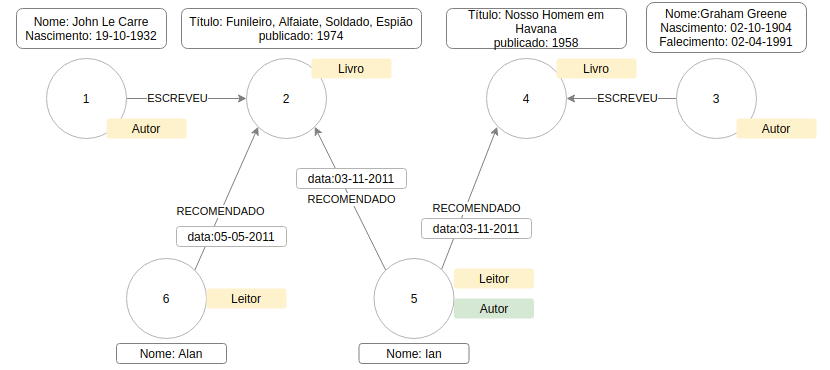
\includegraphics[scale=.50]{./Capitulo3/img/labeled-property-graph-model.png}
         \label{fig:propertygraphmodel}
     \fonte{Labeled Property Graph Model. Adaptado de ~\cite{bruggen:2014}}
 \end{figure}
 
Na Figura~\ref{fig:propertygraphmodel} podem ser identificados os seguintes componentes:

\begin{itemize}
    \item Nós ou Vértices: São utilizados para armazenamento de informações da entidade. Na Figura~\ref{fig:propertygraphmodel} estes são os livros, leitores e autores que estão presentes no modelo.
    
    \item Relacionamentos: São utilizados para conectar nós uns aos outros. Os relacionamentos sempre têm um tipo, um nó inicial e um nó final e uma direção. 
    Eles podem ser auto-referenciados e nunca podem ficar pendurados (faltando nó inicial ou nó final). Figura~\ref{fig:propertygraphmodel} os relacionamentos são representados através das arestas ''ESCREVEU'' e  ''RECOMENDADO''.
    
    \item Propriedades: Propriedades são pares de nome/valor e podem estar presentes e armazenados tanto em nós quanto em relacionamentos. Na Figura~\ref{fig:propertygraphmodel}, ''nome'' e ''nascimento'' são exemplos de propriedades dos nós Autor e Leitor e ''data'' é um exemplo de propriedade do relacionamento ''RECOMENDADO''.
     
    \item Rótulos: Rótulos são um meio eficiente de proporcionar a criação de subgrafos. A atribuição de rótulos aos nós do modelo tem como uma das finalidades principais a simplificação do modelo não sendo mais necessária a criação de uma propriedade de tipo no nó. Rótulos também podem ser utilizados para indexação de informação no banco de dados Neo4J.Na Figura~\ref{fig:propertygraphmodel}, rótulos são representados nos nós por ''Leitor'', ''Livro'' e ''Autor''.

\end{itemize}

Uma das importantes funcionalidades do Neo4J é a utilização de plugins e bibliotecas para consulta ao banco de dados e execução de algoritmos de redes complexas. 
Dentre as várias bibliotecas podemos citar a \emph{Neo4j Graph Algorithms} que fornece um conjunto de procedimentos definidos pelo usuário que podem ser executadas através da linguagem de consulta Cypher.  
A biblioteca \emph{Neo4j Graph Algorithms} \footnote{https://neo4j.com/docs/graph-algorithms/current/} inclui algoritmos para análise de grafos e fluxos de trabalho de aprendizado de máquina com suporte a até dezenas de bilhões de nós e relacionamentos.

Outra biblioteca muito importante utilizada neste trabalho é a \emph{Neo4j Awesome Procedures on
Cypher (APOC)} \footnote{https://neo4j.com/labs/apoc/}. Esta biblioteca consiste em mais de 450 procedimentos e funções que auxiliam tarefas comuns como integração de dados, conversão de tipagem de dados e refatoração de modelos.


\subsection{Apache Spark}


Apache Spark é uma plataforma de processamento e análise de dados em grande escala. 
Ele usa uma abstração de tabela chamada DataFrame para representar e processar dados.
A plataforma integra diversas fontes de dados e suporta linguagens como Scala, Python e R. O Apache Spark fornece algumas bibliotecas, tais como:

\begin{itemize}
    \item Spark SQL: Fornece a capacidade de executar SQL-like queries com a finalidade de consultar e explorar grandes conjuntos de dados.
    
    \item Spark MLIB: Prove algoritmos e pipelines de processamento de apredizado de máquina.
    
    \item Spark Streaming: Prove a capacidade de processamento de dados near real-time.
    
    \item Spark GraphX: Utilizado para processamento de grafos. 
    
\end{itemize}

\subsection{Transformação do \emph{dataset} para a base de dados de grafo do Neo4j}
\label{subsec:work}

A Figura~\ref{fig:workflow} mostra o fluxo de transformação dos dados para a construção do modelo de grafo no Neo4j a partir do \emph{dataset} disponibilizado. Diversos fluxos foram implementados na linguagem Python usando a ferramenta Apache Spark\footnote{https://spark.apache.org/}. 


 \begin{figure}[!h]
 \caption{Fluxo de ingestão de dados}
     \centering
     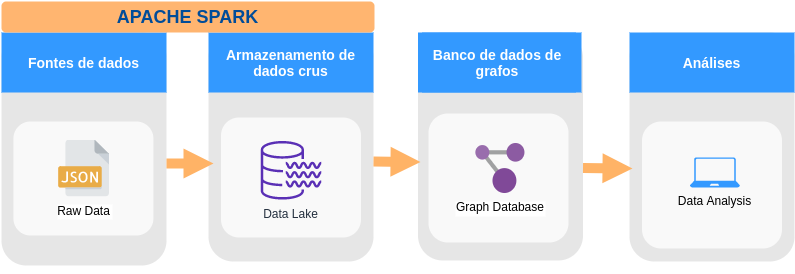
\includegraphics[scale=.45]{./Capitulo3/img/data-flow.png}
         \label{fig:workflow}
     \fonte{Autoria própria}
 \end{figure}
 
 
A primeira etapa consiste no carregamento dos dados brutos (em formato JSON) para uma área de armazenamento (ou \emph{data lake}). Os arquivos JSON são transformados em arquivos parquet\footnote{https://parquet.apache.org/} \cite{Boufea:17} utilizando o Apache Spark. Arquivos parquet são formatos de armazenamento em colunas, otimizados para compressão e rápida recuperação de dados. 
Na sequência, o conteúdo do \emph{data lake} é processado - também usando o Apache Spark - para gerar arquivos no formato CSV com os vértices e arestas do modelo de grafo apresentado na Seção~\ref{sec:met}. 

Diversos fluxos de transformação de dados foram implementados. Detalha-se a seguir as transformações dos dados que criam o vértice \emph{Event} e a aresta \texttt{IS\_NEAR\_BY} do grafo. Estas estruturas modelam a dinâmica de movimentação dos ônibus e justificam o uso de um grafo variante no tempo.

O vértice \emph{Event} é criado a partir da tabela \emph{VEICULOS} (Tabela~\ref{tab:veiculos} ), que contém a geolocalização dos ônibus nos respectivos instantes de tempo. Com essa informação, calcula-se a distância percorrida, o tempo decorrido entre posicionamentos consecutivos e a velocidade média em km/h.


\alt{Se a velocidade for menor do que 15 km/h}, assume-se que houve uma parada do ônibus neste intervalo de tempo e um vértice \emph{Event} é gerado no grafo com os respectivos atributos listados na tabela~\ref{tab:vertice_event}, entretanto com o atributo moving\_status com o valor \emph{STOPPED}.

\alt{Entretanto se a velocidade for maior ou igual a 15 km/h}, assume-se que o veículo está se movimentando, logo são aplicadas as seguintes regras:
 \begin{itemize}
     \item é calculada a média das velocidades posicionadas do veículo entre os vértice \emph{Event} anterior cuja a propriedade moving\_status se encontre com o valor \emph{STOPPED} e o vértice \emph{Event} posterior, também com a propriedade moving\_status com o valor \emph{STOPPED}.
     
     \item é tomado o timestamp médio entre os horários de posicionamento do veículo entre o vértice \emph{Event} anterior cuja a propriedade moving\_status com o valor \emph{STOPPED} e o vértice \emph{Event} posterior, também com a propriedade moving\_status com o valor \emph{STOPPED}
     
     \item é tomado a latitude e longitude média entre posicionamentos do veículo entre o vértice \emph{Event} anterior cuja a propriedade moving\_status  com o valor \emph{STOPPED}  e o vértice \emph{Event} posterior, também com a propriedade moving\_status com o valor \emph{STOPPED}.
     
 \end{itemize}
 Realizados os cálculos é criado um vértice \emph{Event} com o atributo moving\_status com o valor \emph{MOVING}.


A aresta \texttt{IS\_NEAR\_BY} é criada a partir dos vértices \emph{BusStop} e \emph{Event} previamente obtidos das linhas dos ônibus, dos pontos de ônibus e da tabela horária dos ônibus nas linhas (Tabelas~\ref{tab:linhas}, \ref{tab:pontos_linha} e \ref{tab:tabela_veiculo} respectivamente). 

Se uma evento de parada (vértice \emph{Event} com atributo moving\_status com o valor \emph{STOPPED} ) ocorrer a menos de 30 metros de um ponto de ônibus (vértice \emph{BusStop}), considera-se que tal parada ocorreu em um ponto de ônibus e, portanto, cria-se uma aresta \texttt{IS\_NEAR\_BY} para conectar os vértices \emph{Event} e \emph{BusStop} no grafo.

Uma vez construído o banco de dados de grafo para o transporte, consultas e análises de redes complexas podem ser realizadas a partir do Neo4j (\emph{Data Analysis} na Figura~\ref{fig:workflow}).

\section{Análise da integração temporal}
\label{sec:itemporal}

\ric{Aqui precisa detalhar e justificar as decisões feitas para análise}

\ric{Foram selecionadas 15 (ou 30) áreas potenciais para centroides. Criterios para descartar determinadas áreas:
distância entre clusters; proximidade com terminal; efeito corredor; caso Rui Barbosa: as linhas chegam concentradas em um ponto (identificado) e se distribuem na praça.}

\ric{Resumo da metodologia}

\begin{enumerate}
    \item identificam-se os pontos com o maior número de linhas, os quais serão os centroides dos clusters a serem analisados;
    %\item Para cada ponto de ônibus, obtém-se uma série temporal com o número de eventos (paradas de ônibus) em uma janela deslizante de 10 min, calculada minuto a minuto ao longo do período considerado (0 a 24 horas?);
    
    %\item Identificam-se os 10 pontos (centroides) mais bem servidos em termos do número de eventos agregados para todos o período considerado;
    
    \item Para cada centroide, selecionam-se os pontos a uma distância de 600~m do centroide e gera-se uma matriz de correlação entre as séries temporais de cada ponto desta região;
    
    \item Identificam-se os pontos de maior correlação (com o centroide?);
    \item Estes pontos serão os candidatos para estabelecer integração temporal.
\end{enumerate}

\ric{Colocar as decisões tomadas na forma de parâmetros que serão utilizados nos resultados.}

\begin{table}[htb]
    \caption{Parâmetros usados na análise da integração temporal.}
    \centering
    \begin{tabular}{ p{5cm}p{9cm}} 
        \hline
        Parâmetro & Descrição\\
        \hline
        Tamanho da janela & Tamanho da janela deslizante de tempo utilizada para computar o número de paradas em um ponto \\
        Passo da janela & Passo de deslocamento da janela de tempo \\
        Raio do cluster & Área de abrangência de cada centroide ponto de ônibus  \\
        Separação entre clusters  & Distância mínima considerada entre clusters \\
        \hline  
    \end{tabular}
    \label{tab:par}
\end{table}

\section{Sumário do capítulo}

\ric{Destacar os pontos principais do capítulo e eventuais ganchos com outros capítulos.}